This section describes the experiments that uncovers the best combination of hidden layers, neurons and epochs as well as the different strategies. Based on the analysis of wind production from Section~\ref{sec:windPowerAnalysis} the network will try to uncover the best approach to predicting the wind power production. Furthermore, experiments are needed to investigate the influence of data manipulation and statistical inputs as presented in Section~\ref{sec:usingStatisticalInput}. All test results can be seen in Appendix~\ref{sec:windResultsAppendix} and have been carried out naively with only normalization - relevant results will be shown here 

\todo{DRAWING OF NETWORK}

\subsection{Experiment Series One - Selection of input parameters}
The first experiment series is an attempt to find the best constitution of network input parameters based on the analysis in Section~\ref{sec:windPowerAnalysis}. Since the co-relation between wind production and wind speed is very significant it will always be included as a core input parameter in all test combinations.

\subsubsection{Hypothesis}
The analysis in Section~\ref{sec:windPowerAnalysis} showed the co-relation between the different parameters and the wind power production. The most influential factor was as expected wind speed since the wind production directly follows it. Air density and consumption influence wind power production, but they are  both significantly influenced by temperature which makes it an interesting parameter to consider. Wind direction showed connection to wind power production but it needs to be tested in combination with the other inputs to see its potential. The production from the last hour showed not to differ much from the hour to come so this will also be tested as an input parameter.

The most likely input combinations based on the analysis will contain wind speed, air density, time of day, consumption and the last known production.

\subsubsection{Variables}
The variables used in this experiment series:

\begin{itemize}
\item Wind speed (WS)
\item Air density (AD)
\item Consumption (C)
\item Time of day (ToD)
\item Temperature (T)
\item Wind direction (WD)
\item Last known production (L-P)
\item Month (Mo)
\end{itemize}

\subsubsection{Prediction - basic input parameters}
\label{sec:predictionBasicInputParams}
The experiments simulate predictions over the entire year of 2012.

\footnotesize
\begin{center}
\begin{longtable}{|c|c|c|c|c|c|c|c|c|c|c|c|}
\hline
\textbf{WS} & \textbf{AD} & \textbf{C} & \textbf{T} & \textbf{WD} & \textbf{L-P} & \textbf{Mo}& \textbf{ToD} & \textbf{MAE} & \textbf{\% from \#1} & \textbf{H1} & \textbf{H2} \\
\hline
\endfirsthead
\multicolumn{12}{c}%
{\tablename\ \thetable\ -- \textit{Continued from previous page}} \\
\hline
\textbf{WS} & \textbf{AD} & \textbf{C} & \textbf{T} & \textbf{WD} & \textbf{L-P} & \textbf{Mo}& \textbf{ToD} & \textbf{MAE} & \textbf{\% from \#1} & \textbf{H1} & \textbf{H2} \\
\hline
\endhead
\hline \multicolumn{12}{r}{\textit{Continued on next page}} \\
\endfoot
\hline
\endlastfoot
\arrayrulecolor{light-gray}
 \x &  &  &  \x &  &  \x &  &  \x & 127.86 & 0.0\% & 19 & 13 \\ \hline
 \x &  \x &  &  &  \x &  \x &  &  \x & 131.59 & 2.92\% & 20 & 17 \\ \hline
 \x &  \x &  &  &  &  \x &  &  \x & 131.89 & 3.15\% & 16 & 20 \\ \hline
 \x &  \x &  \x &  \x &  \x &  \x &  &  \x & 133.18 & 4.16\% & 13 & 20 \\ \hline
 \x &  \x &  \x &  \x &  \x &  \x &  &  & 133.77 & 4.62\% & 16 & 17 \\ \hline
 \x &  \x &  \x &  &  &  \x &  &  \x & 134.14 & 4.91\% & 12 & 17 \\ \hline
 \x &  \x &  \x &  &  \x &  \x &  &  \x & 135.4 & 5.9\% & 6 & 13 \\ \hline
 \x &  \x &  \x &  &  &  \x &  &  & 136.33 & 6.62\% & 21 & 10 \\ \hline
 \x &  \x &  &  &  &  \x &  \x &  \x & 136.65 & 6.87\% & 5 & 24 \\ \hline
 \x &  &  &  &  &  \x &  &  & 137.33 & 7.41\% & 9 & 15 \\ \hline
 . & . & . & . &  .  & . &  . & . & . & . \\ 
 . & . & . & . &  .  & . &  . & . & . & . \\ 
 . & . & . & . &  .  & . &  . & . & . & .\\ \hline
 \x &  \x &  &  \x &  &  \x &  \x &  & 170.93 & 33.69\% & 9 & 18 \\ \hline
 \x &  &  \x &  \x &  \x &  \x &  \x &  \x & 171.61 & 34.22\% & 9 & 13 \\ \hline
 \x &  &  \x &  \x &  &  \x &  \x &  & 172.72 & 35.09\% & 14 & 15 \\ \hline
 \x &  &  &  &  \x &  \x &  \x &  & 173.12 & 35.4\% & 18 & 90 \\ \hline
 \x &  &  \x &  \x &  &  \x &  \x &  \x & 173.65 & 35.81\% & 13 & 17 \\ \hline
 \x &  \x &  \x &  \x &  \x &  \x &  \x &  \x & 174.26 & 36.29\% & 15 & 14 \\ \hline
 \x &  \x &  &  \x &  &  \x &  \x &  \x & 174.55 & 36.52\% & 3 & 17 \\ \hline
 \x &  &  &  \x &  &  \x &  \x &  \x & 174.85 & 36.75\% & 1 & 17 \\ \hline
 \x &  \x &  \x &  &  \x &  \x &  \x &  & 180.89 & 41.48\% & 20 & 11 \\ \hline
 \x &  \x &  &  &  \x &  \x &  \x &  \x & 199.22 & 55.81\% & 18 & 19 \\ \hline
\caption{Wind Production Input Parameter Test Top and bottom 10. It is based on 3 month of historical data and 200 epochs. It is an average of the prediction over 8000 hours}
\label{table:windProdInputParamsTop10}
\end{longtable}
\end{center}
\normalsize

To make sure that the top-3 is not a case of randomization they have all been run on the same year 10 times which can be seen in Table \todo{create it}


All results from the first experiment can be seen in Appendix~\ref{sec:simpleInputTest}. The results vary from the best MAE at 127,86 to the worst being 199,22. Top and bottom 10 is shown sorted in Table~\ref{table:windProdInputParamsTop10}. The appendix shows that when wind speed is used as the only input parameter the MAE is 149,72. This illustrates the expected relationship between wind speed and wind production. The experiment further indicates that time of day, air density and last production are significant. This correspond well with the analysis in Section~\ref{sec:windPowerAnalysis} where the relationship between wind production and the parameters are established. The analysis concerning wind production development is seen in the experiments where it is included it all of top 10. The production does not differ much from one hour to the next which is reflected in the last known production input parameter --- more sophisticated attempts with statistic will be in experiments to come. The development is also represented in the bottom which will be addressed when discussing month as input. What comes as a surprise is the under-representation of consumption in top 10 because the analysis showed a good co-relation. A possible explanation can be the substitution with temperature which highly influences consumption as discussed in the analysis section. Temperature is also the significant factor in calculating air density since pressure is close to constant as described in Section~\ref{sec:airDensity} --- this might explain why rank top-3 is without consumption and why air density can substitute consumption.

Wind Direction is represented four times in top 10. What is noticeable is the same combinations without wind direction is also represented which indicates the indifference of wind direction, e.g. see \#2-\#3 and \#6-\#7 with only little difference between them. This is further backed up by the analysis which only showed a low co-relation. 

The contributory cause to the bad accuracy in the bottom is month and how it in general does not help the prediction when using it together with a dataset containing only 3 months. Month represents the seasonal perspective of the input parameters and is suppose to find the relationship between months and the production in general. Since the historical data used for prediction is only 3 months, it does not capture how all the same month last year influenced the production. In the case of wind power prediction it seems to creating more noise and thereby affect the prediction badly. A possible solution to obtain the seasonality aspect is presented in\cite{pjmForecast} where the Neural Network is trained with 45 days from before the day to be predicted, and 45 days before and after in the previous year. By using this approach the month parameter will reflect the influence of the months around you from the last year. This needs validation in an prediction for itself.

\subsubsection{Prediction - Seasonal aspect}
Experiment two will uncover and discuss the seasonal aspect when used as input parameter and how it relates to the size of the dataset. The experiment results can be seen in Appendix~\ref{sec:simpleInputTestSeason} and top-10 in Table~\ref{table:seasonalWindProdInputParamsTop10}. The results show a decrease in MAE which can be explained by the increased data size of the training set that makes it harder for the ANN to generalize. According to\cite{1} too large training sets should be avoided because it has a tendency to be overtrained --- this can be backed up by the close results in top-10 that only differs to a maximum of 1,12\%. The network generalizes on much more data and if some values only influence the wind production in smaller periods of the year it will be suffocated between the ones that are import over the entire year. Wind speed is significant over the entire year and by itself got a MAE of 149,72 as described in Section~\ref{sec:predictionBasicInputParams} and the answer could be that the network over-trains itself by dedicating to much responsibility to wind speed because it in general is the most important input. 
Furthermore, the possible benefits from including the seasonal aspect when predicting wind production can not make up for the loss in accuracy by the increase in the size of training data. It is further seen that month is only represented once in top 10. To validate the decrease in accuracy the date has been a prediction has been conducted with a training set of an entire year and the result can be seen in Table~\ref{table:seasonWindProdInputParamsTop2WholeYear}. The MAE is around the same but instead it takes longer time to process when training on an entire year which makes the small dataset an even better choice --- processing time will be discussed in more details in experiments to come. The usage of only 3 months in the dataset can also be argued to contain the seasonal aspect for the hours to predict. The three months in the set will reflect the current season that you are in and therefore adding more data will only create more noise. When the month parameters is used on only three months it will only reflect how the impact of the past months but not the one that you are going into --- it will not be able to say anything about the beginning of a month because it has never seen such a month before. Furthermore, it is hard to generalize upon a few days (impossible the first day) in a month and therefore the input parameter will be highly influenced by the month before which can become problematic when seasons are shifting.

It needs to be made clear that it is one input parameter of the entire network. The above discussion illustrates that the small dataset itself contains the seasonality aspect since the network trains and generalizes only upon the current season --- it knows of nothing more and for this reason the month parameter will be omitted in the prediction of wind production. It can be further backed up by Table~\ref{table:windProdInputParamsTop10} where only one with month as input is represented but all of bottom 10 is with. 

In experiments concerning prediction of wind production the month input parameter will be left out.  

\footnotesize
\begin{center}
\begin{longtable}{|c|c|c|c|c|c|c|c|c|c|c|c|}
\hline
\textbf{WS} & \textbf{AD} & \textbf{C} & \textbf{T} & \textbf{WD} & \textbf{L-P} & \textbf{Mo}& \textbf{ToD} & \textbf{MAE} & \textbf{\% from \#1} & \textbf{H1} & \textbf{H2} \\
\hline
\endfirsthead
\multicolumn{12}{c}%
{\tablename\ \thetable\ -- \textit{Continued from previous page}} \\
\hline
\textbf{WS} & \textbf{AD} & \textbf{C} & \textbf{T} & \textbf{WD} & \textbf{L-P} & \textbf{Mo}& \textbf{ToD} & \textbf{MAE} & \textbf{\% from \#1} & \textbf{H1} & \textbf{H2} \\
\hline
\endhead
\hline \multicolumn{12}{r}{\textit{Continued on next page}} \\
\endfoot
\hline
\endlastfoot
\arrayrulecolor{light-gray}
 \x &  \x &  \x &  &  \x &  \x &  &  \x & 142.88 & 0.0\% & 7 & 17 \\ \hline
 \x &  &  &  \x &  \x &  \x &  &  & 142.89 & 0.01\% & 14 & 11 \\ \hline
 \x &  \x &  &  &  \x &  \x &  &  \x & 143.37 & 0.34\% & 6 & 21 \\ \hline
 \x &  \x &  \x &  \x &  \x &  \x &  &  \x & 143.97 & 0.76\% & 8 & 25 \\ \hline
 \x &  &  &  &  &  \x &  &  \x & 143.98 & 0.77\% & 5 & 21 \\ \hline
 \x &  \x &  \x &  \x &  &  \x &  \x &  & 144.11 & 0.86\% & 6 & 17 \\ \hline
 \x &  \x &  &  &  &  \x &  &  & 144.12 & 0.87\% & 7 & 12 \\ \hline
 \x &  &  &  &  &  &  &  \x & 144.28 & 0.98\% & 12 & 17 \\ \hline
 \x &  &  \x &  &  \x &  \x &  &  & 144.42 & 1.08\% & 11 & 10 \\ \hline
 \x &  \x &  &  \x &  \x &  \x &  &  \x & 144.48 & 1.12\% & 4 & 17 \\ \hline
\caption{Top 10 seasonal wind production test. It is based on 3 month of historical data and one month after from the previous year. It is run with 200 epochs and predicts 8000 hours in 2012}
\label{table:seasonalWindProdInputParamsTop10}
\end{longtable}
\end{center}
\normalsize

\todo{trend discussion in relation to why seasonal impl is better on small dataset}.

\footnotesize
\begin{center}
\begin{longtable}{|c|c|c|c|c|c|c|c|c|c|c|}
\hline
\textbf{WS} & \textbf{AD} & \textbf{C} & \textbf{T} & \textbf{WD} & \textbf{L-P} & \textbf{Mo}& \textbf{ToD} & \textbf{MAE} & \textbf{H1} & \textbf{H2} \\
\hline
\endfirsthead
\multicolumn{11}{c}%
{\tablename\ \thetable\ -- \textit{Continued from previous page}} \\
\hline
\textbf{WS} & \textbf{AD} & \textbf{C} & \textbf{T} & \textbf{WD} & \textbf{L-P} & \textbf{Mo}& \textbf{ToD} & \textbf{MAE} & \textbf{H1} & \textbf{H2} \\
\hline
\endhead
\hline \multicolumn{11}{r}{\textit{Continued on next page}} \\
\endfoot
\hline
\endlastfoot
\arrayrulecolor{light-gray}
 \x &  \x &  \x &  \x &  &  \x &  \x &  & 147.98 & 6 & 22 \\ \hline
\caption{Seasonal wind production test based on an entire year. It is run with 200 epochs and predicts 8000 hours in 2012}
\label{table:seasonWindProdInputParamsTop2WholeYear}
\end{longtable}
\end{center}
\normalsize
\todo{see appendix}

\subsubsection{Conclusion}
The expectation was that the best input combinations contained wind speed, air density, consumption, time of day and last hour production. Wind speed, last production, air density and time of day showed to be highly represented in Table~\ref{table:windProdInputParamsTop10} which indicates and supports the good co-relation to wind power production. Surprisingly, consumption was not represented in top-3. Temperature came to mind as an explanation since it influences both air density and consumption a great deal and therefore could be a substitute for both. Air density is calculated with temperature which explains why it can substitute consumption.

The first 175 hours of the best prediction from Table~\ref{table:windProdInputParamsTop10} can be seen in Figure~\ref{fig:bestInputParameterPrediction}. It can be observed that the prediction follows the trend of the actual wind production. The obvious challenge is that the prediction takes time to identify shifting trend --- either it identifies it before happens or after it happened. From hour 25-50 it is way behind the actual slope. It can also be seen around hour 100-110 that it significantly overshoots and in 120-160 undershoots its target before actually identifying the shift. The statistical approach described in Section~\ref{sec:usingStatisticalInput} can possible help in these cases by taking current trend into consideration. Experiments will take up this approach for comparison.  

\begin{figure}[H]
\centering
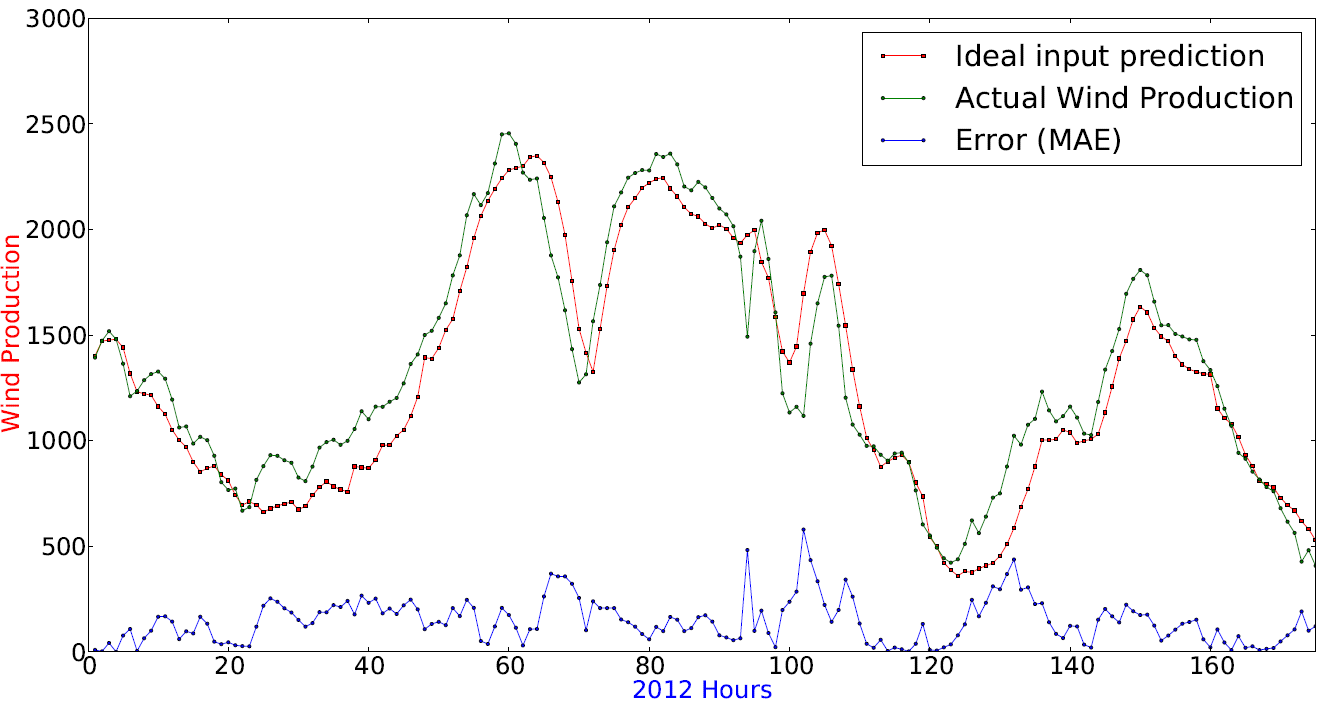
\includegraphics[width=0.99\linewidth]{billeder/bestInputParameterPrediction.png}
\caption{Wind production prediction for 175 hours in 2012}
\label{fig:bestInputParameterPrediction}
\end{figure}   

The experiments to come will be based on input combinations from the top 3 from Table~\ref{table:windProdInputParamsTop10}. The inputs are:
\begin{itemize}
\item Wind speed;
\item Air density;
\item Wind Direction;
\item Temperature;
\item Last known production;
\item Time of day;
\end{itemize}

\todo{Talk about the network size}

\subsection{Experiment Two - Data Manipulation}
Experiment two tries to discover the best ways to represent the input data. The need for manipulating the data can arise if irregularities exist that cannot be predicted or simply to adjust the data to better fit the inner workings of the neural network. The 3 approaches to data manipulation used in this thesis is normalization, trimming and using a matrix as input. The necessity is described in more detail in Section~\ref{sec:DataManipulation}. Normalization is necessary for all input and was also used in experiment one. Trimming is used to trim away irregularities if such exist but it does not apply for when predicting wind power production \todo{create this in the analysis}. The purpose of the experiments in series two is to turn inputs into a matrix whenever it makes sense. As described in Section~\ref{sec:Matrix} one input parameter is split into a input parameter for all of its possible values. Each value then has a weight that is adjusting itself according to the error as illustrated in Section~\ref{sec:annSection}. This is of course only an option if all values are known in advance and of a manageable size. When considering wind production forecasting this is valid for hours of the day, month and wind speed. Only wind speed and time of day will be tested here due to the omitting of the month parameter in experiment series one.

\subsubsection{Hypothesis} 
The matrix manipulation makes sense when values are equally distributed as discussed in Section~\ref{sec:Matrix}. This apply for time of day and therefore it is expected to see an improvement when matrix is applied here. This is not the case for wind speed and the expectation is instead to see a worse result when applying matrix.

\subsubsection{Prediction - Applying matrix}
The decrease in accuracy when using wind speed as a matrix can be seen in Table~\ref{windProdInputParamsTop10WithMatrix}. None of the best results contain wind speed as matrix and only differ 3,02\% from the top result whereas the results with wind speed as matrix lies between 7,49\% and 23,14\%. The best result is the same as in Table~\ref{table:windProdInputParamsTop10} but number \#2 and \#3 has switched places but the difference between them is still not that significant. All in top-3 improved with an average improvement of 1,3\%.  


\begin{center}
\begin{longtable}{|c|c|c|c|c|c|c|c|c|c|c|}
\hline
\textbf{WS} & \textbf{AD} & \textbf{C} & \textbf{T} & \textbf{WD} & \textbf{L-P} & \textbf{ToD} & \textbf{MAE} & \textbf{\% from \#1} &  \textbf{H1} & \textbf{H2}  \\
\hline
\endfirsthead
\multicolumn{11}{c}%
{\tablename\ \thetable\ -- \textit{Continued from previous page}} \\
\hline
\textbf{WS} & \textbf{AD} & \textbf{C} & \textbf{T} & \textbf{WD} & \textbf{L-P} & \textbf{ToD} & \textbf{MAE} & \textbf{\% from \#1} &  \textbf{H1} & \textbf{H2}  \\
\hline
\endhead
\hline \multicolumn{11}{r}{\textit{Continued on next page}} \\
\endfoot
\hline
\endlastfoot
\arrayrulecolor{light-gray}
 \x &  &  &  \x &  &  \x &  \x (m) & 126,25 & 0,0\% & 18 & 17 \\ \hline
 \x &  \x &  &  &  &  \x &  \x (m) & 127,95 & 1,35\% & 13 & 19 \\ \hline
 \x &  \x &  &  &  \x &  \x & \x (m) & 130,07 & 3,02\% & 2 & 23 \\ \hline
 \x (m) & &  &  \x &  &  \x &  \x (m) & 135,71 & 7,49\% & 13 & 16 \\ \hline
 \x (m) & \x &  &  &  \x &  \x &  \x & 144,44 & 14,41\% & 14 & 12 \\ \hline
  \x (m) & \x &  &  &  &  \x &  \x & 147,63 & 17,12\% & 8 & 16 \\ \hline
 \x (m) & \x &  &  &  \x &  \x &  \x (m) & 149,18 & 18,16\% & 13 & 21 \\ \hline
 \x (m) & &  &  \x &  &  \x &  \x & 149,19 & 18,17\% & 10 & 22 \\ \hline
 \x (m) & \x &  &  &  &  \x &  \x (m) & 155,46 & 23,14\% & 16 & 13 \\ \hline
\caption{Matrix test}
\label{table:windProdInputParamsTop10WithMatrix}
\end{longtable}
\end{center}

\subsubsection{Conclusion}
The hypothesis concerning the decrease in performance when applying matrix to wind speed is obvious from the results in Table Table~\ref{windProdInputParamsTop10WithMatrix}. Wind speeds are represented by 41 different values in our data set. Instead of having only one input to represent each of the values, the matrix turned into 41 inputs for every single value. The purpose is to have a weight that tells exactly how much the specific wind speed in general influence the wind production to predict. The network will do so by adjusting a weight for the different wind speeds in the matrix whenever they are seen. As described in Section~\ref{sec:Matrix} a problem arise if some values does not exist or are under-represented. This will cause that specific value to be under-expressed because the weight has only been adjusted a few times or not at all. The seasonal differences in wind power production is described in Section~\ref{sec:windProdSeasonality} and since wind production follows wind speed it can be considered very likely that the training set of only 3 months does not cover all wind speeds for all predictions.

The other hypothesis was regarding the improvement of matrix on time of day. All predictions with only time of day as a matrix outperformed all other in terms of accuracy in this experiment. The matrix time of day predictions are all better than their corresponding prediction in Table~\ref{table:windProdInputParamsTop10}. The improvement was in average only 1,3\% which is not very significant and it can therefore be argued if matrix is worth the enlargement in input parameters. Trade-offs must be made in relation to the time and the achieved improvement. The trade-off between time and inputs will be discussed further in a later experiment but under the current circumstances of our test procedure from Section~\ref{sec:testProcedure} we will move on with the time of day as matrix.    \todo{is this valid enough? We current assume the 8000 hours to be general and therefore 1,3\% is valid and better than none}.

\subsection{Experiment Series Three - Calculated Inputs}
This subsection is experimenting with the concepts described in Section~\ref{sec:usingStatisticalInput}. The point is to add inputs that in some way analyse productions from past hours to help the existing generalization approach its target more accurately. We therefore see it as independent from the input analysis since it will help the best of the input combinations to perform better. All of the approaches takes outset in previous hours so the first step is to find the best number of hours to calculate upon. The different approaches are historical volatility, skewness, simple curve analysis and inclusion of previous productions as input. 

\subsubsection{Historical Volatility}
Historical Volatility is presented in Section~\ref{sec:usingStatisticalInput}. It will calculate the volatility of the productions from hour to hour. This means that the last hour in the training set will hold information of the volatility of the entire dataset. We will use the EWMA to calculate volatility \todo{ref it back} and here it is necessary to experiment with the correct decay rate. The EWMA will always include the last hours EWMA --- this is why it is called moving average. The test will be performed in the best MAE from last experiment. When the best rate has been established for hour dataset it will be tested on top 10 from Table~\ref{table:windProdInputParamsTop10} with and without matrix.

\begin{center}
\begin{longtable}{|c|c|}
\hline
\textbf{Devay} & \textbf{MAE} \\
\hline
\endfirsthead
\multicolumn{2}{c}%
{\tablename\ \thetable\ -- \textit{Continued from previous page}} \\
\hline
\textbf{Decay} & \textbf{MAE}\\
\hline
\endhead
\hline \multicolumn{2}{r}{\textit{Continued on next page}} \\
\endfoot
\hline
\endlastfoot
\arrayrulecolor{light-gray}
0,10 & 122,75 \\ \hline
0,30 & 125,49 \\ \hline
0,60 & 127,49 \\ \hline
0,70 & 127,97 \\ \hline
0,50 & 130,47 \\ \hline
0,20 & 134,06 \\ \hline
0,80 & 135,17 \\ \hline
0,40 & 137,21 \\ \hline
0,90 & 139,16 \\ \hline
\caption{Different decay rates for historical volatility}
\label{table:historicalVoltalityHours}
\end{longtable}
\end{center}

\subsubsection{Skewness}
Skewness is a calculation of how much a distribution leans to one side of the mean \todo{write some about it in the statistics section}. What is important to locate is how many previous hours to include in the calculation of the skew. Table~\ref{table:skewnessHours} shows results where the best fit is found to be 16 hours. This will be basis for further testing when trying to use the methods in combination to see if any of them can augment each other. At first glance skewness seems to be indifferent in the case of wind production.

\begin{center}
\begin{longtable}{|c|c|}
\hline
\textbf{Hours} & \textbf{MAE} \\
\hline
\endfirsthead
\multicolumn{2}{c}%
{\tablename\ \thetable\ -- \textit{Continued from previous page}} \\
\hline
\textbf{Hours} & \textbf{MAE}\\
\hline
\endhead
\hline \multicolumn{2}{r}{\textit{Continued on next page}} \\
\endfoot
\hline
\endlastfoot
\arrayrulecolor{light-gray}
16 & 125.85 \\ \hline
4 & 127.52 \\ \hline
24 & 129.63 \\ \hline
8 & 131.18 \\ \hline
12 & 131.26 \\ \hline
6 & 131.51 \\ \hline
20 & 134.81 \\ \hline
2 & 139.33 \\ \hline
\caption{Prediction With Skewness and different hours}
\label{table:skewnessHours}
\end{longtable}
\end{center}

\subsubsection{Curve Analysis}
Curve analysis covers basic slope calculation of the curve. The intention is to get a notion of how much the previous productions was going upwards before the current hour. The purpose is to capture how the slopes in general relates to the production --- when we have a very steep slope how does that in general affect the production. Table~\ref{table:curveAnalysisHours} clearly shows that the curve analysis does not work as intended. \todo{show graph}.

\begin{center}
\begin{longtable}{|c|c|}
\hline
\textbf{Hours} & \textbf{MAE} \\
\hline
\endfirsthead
\multicolumn{2}{c}%
{\tablename\ \thetable\ -- \textit{Continued from previous page}} \\
\hline
\textbf{Hours} & \textbf{MAE} \\
\hline
\endhead
\hline \multicolumn{2}{r}{\textit{Continued on next page}} \\
\endfoot
\hline
\endlastfoot
\arrayrulecolor{light-gray}
20 & 133.27 \\ \hline
16 & 133.52 \\ \hline
12 & 137.05 \\ \hline
8 & 140.0 \\ \hline
24 & 146.5 \\ \hline
6 & 148.5 \\ \hline
2 & 151.62 \\ \hline
4 & 161.12 \\ \hline
\caption{Curve Analysis on different hours}
\label{table:curveAnalysisHours}
\end{longtable}
\end{center}
\normalsize

\subsubsection{Combining the approaches}
All of the results in the table.

\begin{center}
\begin{longtable}{|c|c|}
\hline
\textbf{Hours} & \textbf{MAE} \\
\hline
\endfirsthead
\multicolumn{2}{c}%
{\tablename\ \thetable\ -- \textit{Continued from previous page}} \\
\hline
\textbf{Hours} & \textbf{MAE} \\
\hline
\endhead
\hline \multicolumn{2}{r}{\textit{Continued on next page}} \\
\endfoot
\hline
\endlastfoot
\arrayrulecolor{light-gray}
Volatility with 0,10 decay & 122,75 \\ \hline
Skewness with 16 hours & 125.85 \\ \hline
Scatter of prices & 134.7 \\ \hline
Curve Analysis with 20 hours & 133.27 \\ \hline
\caption{Comparison of the approaches}
\label{table:comparisonStatistics}
\end{longtable}
\end{center}

\todo{say something clever about them}.
Also tried scatter as presented~\cite{singhal2011electricity} which achieved a MAE of 134.7 and way behind the other approaches. A combination of all is illustrated in Table~\ref{table:idealCombination}. \todo{something clever should be written}

\footnotesize
\begin{center}
\begin{longtable}{|c|c|c|c|c|}
\hline
\textbf{Volatility} & \textbf{Skewness} & \textbf{Scatter} & \textbf{Curve} & \textbf{MAE} \\
\hline
\endfirsthead
\multicolumn{5}{c}%
{\tablename\ \thetable\ -- \textit{Continued from previous page}} \\
\hline
\textbf{Volatility} & \textbf{Skewness} & \textbf{Scatter} & \textbf{Curve} & \textbf{MAE} \\
\hline
\endhead
\hline \multicolumn{5}{r}{\textit{Continued on next page}} \\
\endfoot
\hline
\endlastfoot
\arrayrulecolor{light-gray}
 \x &  \x &  &  & 118.17 \\ \hline
 \x &  \x &  &  \x & 122.77 \\ \hline
 &  &  &  & 125.65 \\ \hline
 \x &  \x &  \x &  & 129.24 \\ \hline
 &  \x &  \x &  & 130.02 \\ \hline
 \x &  &  &  \x & 131.54 \\ \hline
 &  &  &  \x & 132.29 \\ \hline
 &  &  \x &  & 132.31 \\ \hline
 \x &  &  \x &  & 132.55 \\ \hline
 \x &  &  &  & 133.73 \\ \hline
 &  \x &  &  & 134.61 \\ \hline
 &  \x &  &  \x & 140.49 \\ \hline
 &  \x &  \x &  \x & 140.66 \\ \hline
 \x &  &  \x &  \x & 140.69 \\ \hline
 \x &  \x &  \x &  \x & 150.24 \\ \hline
 &  &  \x &  \x & 153.8 \\ \hline
\caption{All combinations of statistical features on the best from matrix}
\label{table:idealCombination}
\end{longtable}
\end{center}
\normalsize

Table~\ref{table:topFromMatrixWithStatistics} shows the two top combinations applied on the top 3 input combinations with matrix from Table~\ref{table:windProdInputParamsTop10WithMatrix}. It is first of all noticeable that the top 3 positions are the same as in all of the combination tests. Secondly, the results are in general improved. The best from ~\ref{table:idealCombination} is the same as the best ranked here. The results are equal which again emphasizes the ranking and the input combination. \todo{re-articulate/rephrase and say more stuff}.     

\begin{center}
\begin{longtable}{|c|c|c|c|c|c|c|c|c|c|c|c|}
\hline
\textbf{WS} & \textbf{AD} & \textbf{C} & \textbf{T} & \textbf{WD} & \textbf{L-P} & \textbf{ToD} & \textbf{Vola} & \textbf{Skew} & \textbf{Scat} & \textbf{Curve} & \textbf{MAE} \\
\hline
\endfirsthead
\multicolumn{12}{c}%
{\tablename\ \thetable\ -- \textit{Continued from previous page}} \\
\hline
\textbf{WS} & \textbf{AD} & \textbf{C} & \textbf{T} & \textbf{WD} & \textbf{L-P} & \textbf{ToD} & \textbf{Vola} & \textbf{Skew} & \textbf{Scat} & \textbf{Curve} & \textbf{MAE} \\
\hline
\endhead
\hline \multicolumn{12}{r}{\textit{Continued on next page}} \\
\endfoot
\hline
\endlastfoot
\arrayrulecolor{light-gray}
 \x &  &  &  \x &  &  \x &  \x (m) & \x &  \x &  &  & 119.84 \\ \hline
 \x &  \x &  &  &  &  \x &  \x (m) & \x &  \x &  &  & 124.31 \\ \hline
 \x &  \x &  &  &  \x &  \x &   \x (m) & \x &  \x &  &  & 125.69 \\ \hline
 \x &  \x &  &  &  \x &  \x &  \x (m) & \x &  \x &  &  \x & 127.42 \\ \hline
 \x &  &  &  \x &  &  \x &  \x (m) & \x &  \x &  &  \x & 128.19 \\ \hline
 \x &  \x &  &  &  &  \x &  \x (m) & \x &  \x &  &  \x & 130.19 \\ \hline
\caption{Top 3 tested with the two ideal statistics setting}
\label{table:topFromMatrixWithStatistics}
\end{longtable}
\end{center}


\todo{better with or without trimming?}


\todo{do 1-12-24 step ahead to show the "carry-with"-error} 


\subsection{Experiment Three - Prediction Strategies}
Similar days, the use of more than one neural network to "re-calculate" results. Try other training algorithm. Try recurrent network.

The re-calculation concept works by letting other neural networks re-calculate the prediction from the original network. The purpose is to identify places where the generalization function has problems and then divide it into new neural networks that only have the purpose of focusing on these problematic situations. For simplicity we are going to apply this to the small numbers and big numbers of the dataset. We will define what is small and big by taking the 2 and 98 percentile. Whenever the "original" network predicts something in or close to the big or small interval then the responsibility of that prediction is forwarded to one of the two. It works like a second opinion but here the network has been specialized to only focus on a specific part of the dataset instead of everything\todo{give example of corrections}. It creates a normalization function on a smaller dataset and leaves out a lot of unnecessary information. It does not need to account for anything other than its interval in the generalization function so it should be able to predict its target group better. What is smart about the second opinion is that we let the original network decide if it actually thinks we are in the low numbers --- if we are then we can possibly make that prediction even more accurate. These thoughts could basically we applied on all other parts of possible wind production values. 

The problem can be if the intervals are too small which will cause the dataset to be too small and hard for the ANN to generalize upon. This was the same problem seen with matrix and wind speeds \todo{elaborate}. Some periods can be with only a few small or big values and then the network will have a hard time predicting values if we are moving into a periods with a lot. Another problem is that you are basically chopping up the curves under or above a predefined number (98 or 2 percentile) (or this is a problem at all?). Another thing is the decrease in performance because you have to train and instantiate the number of new networks. Trade-off.

\begin{center}
\begin{longtable}{|c|c|}
\hline
\textbf{Strategy} & \textbf{MAE} \\
\hline
\endfirsthead
\multicolumn{2}{c}%
{\tablename\ \thetable\ -- \textit{Continued from previous page}} \\
\hline
\textbf{Strategy} & \textbf{MAE} \\
\hline
\endhead
\hline \multicolumn{2}{r}{\textit{Continued on next page}} \\
\endfoot
\hline
\endlastfoot
\arrayrulecolor{light-gray}
Small and Big ANN strategy & 190.01 \\ \hline
Small and big with Similar Days & 137.61 \\ \hline
Just similar days and ideal inputs & 138.93 \\ \hline
Hybrid training strategy (Levenberg-Marquat) & 142.07 \\ \hline
Tried with recurrent neural network & 211.12 \\ \hline
\caption{Strategies}
\label{table:strategiesOnIdeal}
\end{longtable}
\end{center}

The small and big ann is so close to the result with the strategy. It is hard to say if it is improved. The reason lays in the relatively small interval they are focusing on (Small being from 0-60 and big being 1950-maximum). To see the real potential in this approach more intervals need to be included and more testing is needed. \todo{hmm, try on only big because that should be the obvious result in MAE}.

\todo{fix table so that it makes more sense}
Problems with similar days is that it does not see the whole picture. The problem arises when only a few similar days exist in the last 3 months \todo{show}. Then it will be hard to generalize upon, especially if all other days are pulling the production in a other direction than the similar days. The similar days approach should be tested on an entire year.


\subsection{Experiment Four - Black Box Optimization}
Epochs, use 